\documentclass[10pt,conference]{IEEEtran}

% Paquetes
\usepackage[utf8]{inputenc}
\usepackage[spanish,es-tabla]{babel} % Idioma español con tablas
\usepackage{apacite} % Referencias y Citas
\usepackage{float} % Para var H, figure
%\usepackage{subcaption}
\usepackage{graphicx}  % Paquete para insertar figuras
%\usepackage{subfigure} % imagenes multiples
\usepackage{url}
\usepackage{amsmath}%Paquete para insertar símbolos matemáticos
\usepackage{newtxmath}
\usepackage{multirow}
\usepackage[table,xcdraw]{xcolor}
%---------- pie de pagina
\usepackage{fancyhdr}
\pagestyle{fancy}
\fancyhf{}
\rfoot[]{\thepage}
\usepackage{ragged2e} % \justify
%-----------------

%-------------------------------------------------------------
% APA7 CITAS
% \citeA{autor} -> Autor (año)
% \cite[p.~11]{autor}. cita corta -40 words -> (Autor, año, página)
%-------------------------------------------------------------

%Para alinear 4 y 5 autor.
\makeatletter
\newcommand{\newlineauthors}{%
  \end{@IEEEauthorhalign}\hfill\mbox{}\par
  \mbox{}\hfill\begin{@IEEEauthorhalign}}
\makeatother
%----------------------------------------------

\title{ Simulador virtual de Máquina Expendedora de Productos de Protección Personal contra el Covid-19 usando Autómata Finito en Java}

\author{\IEEEauthorblockN{1\textsuperscript{ero} Fabricio Julian}
\IEEEauthorblockA{\textit{Escuela de Informática} \\
\textit{Universidad Nacional de Trujillo}\\
Trujillo, Perú \\
t452700220@unitru.edu.pe}
\and
\IEEEauthorblockN{2\textsuperscript{do} Angely Mendez}
\IEEEauthorblockA{\textit{Escuela de Informática} \\
\textit{Universidad Nacional de Trujillo}\\
Trujillo, Perú \\
t052701020@unitru.edu.pe}
\and
\IEEEauthorblockN{3\textsuperscript{ero} Ciara Mendez}
\IEEEauthorblockA{\textit{Escuela de Informática} \\
\textit{Universidad Nacional de Trujillo}\\
Trujillo, Perú \\
t022700920@unitru.edu.pe}
\and
\newlineauthors
\IEEEauthorblockN{4\textsuperscript{to} Valentina Padilla}
\IEEEauthorblockA{\textit{Escuela de Informática} \\
\textit{Universidad Nacional de Trujillo}\\
Trujillo, Perú \\
t032700320@unitru.edu.pe}
\and
\noindent
\IEEEauthorblockN{5\textsuperscript{to} Angie Recalde}
\IEEEauthorblockA{\textit{Escuela de Informática} \\
\textit{Universidad Nacional de Trujillo}\\
Trujillo, Perú \\
t512700720@unitru.edu.pe}
}

\begin{document}
\renewcommand{\BOthers}[1]{et al.\hbox{}} % Para reemplazar y cols. por et.al (=+ de 3 autores) APA7
\renewcommand{\IEEEkeywordsname}{{\bfseries Palabras claves:}} % Colocar Keywords en Spanish

\maketitle

\begin{abstract}
En el presente artículo se desarrolla y se describe la elaboración de un prototipo del simulador virtual de una máquina expendedora de productos de protección personal que ante la actual crisis sanitaria que se está viviendo que es el COVID-19 se considera de suma importancia contribuyendo así al autocuidado personal, evitar la propagación del virus y sin causar aglomeraciones innecesarias en las farmacias por la compra de estos artículos. El prototipo se desarrollará mediante el diseño de un Autómata Finito atribuyendo al funcionamiento del simulador de máquina expendedora y en el lenguaje de programación de Java.
\end{abstract}

\vspace{2mm}
\begin{IEEEkeywords}
Autómatas finitos, máquina, bioseguridad. 
\end{IEEEkeywords}

\vspace{1mm}
\section{\textbf{Introducción}}
La pandemia actual en la que como sociedad estamos sumergidos y viviendo, ha generado muchas muertes y graves secuelas en la salud. Por lo que muchas instituciones y los gobiernos motivan un mayor auto cuidado para prevenir contagios de coronavirus realizando recomendaciones y estrategias; la recomendación principal y en la que hacen énfasis es mantener el distanciamiento social y utilizar artículos de protección personal en cualquier lugar público.

Por lo señalado  anteriormente, de la importancia de estar protegidos en lugares concurridos, se considera a las máquinas dispensadoras, para que asuman su rol, pensando en la practicidad y facilidad de adquirir uno o varios productos, permitiendo una compra rápida sin intermediarios, sin restricciones de tiempo evitando las aglomeraciones, largas colas y contagios por la Covid-19.

Por ello en el presente artículo, se explica sobre un prototipo de Simulador Virtual de Máquina Expendedora de Productos de Protección Personal contra el Covid-19 usando Autómata Finito, este es oportuno en el proceso que realiza la máquina cuando interactúa con el usuario, desde recibir el dinero hasta la entrega del producto elegido, en el lenguaje de programación Java. Además se detalla la realidad problemática, los antecedentes, los objetivos general y específicos, el alcance y limitaciones. Añadiendo también el análisis inicial, el diseño detallado, los resultados obtenidos, la discusión y finalmente se presenta una breve conclusión.

\vspace{1mm}    
\section{\textbf{Generalidades}}

\vspace{2mm}
\subsection{\underline{\textbf{Realidad problemática}}}

El SARS-COV 2, más conocido como el COVID-19, una enfermedad infecciosa, donde la mayoría de personas infectadas por este virus experimentan una enfermedad respiratoria, leve o crónica, las personas llegan a perder la vida, para ello la mejor manera de prevenir la enfermedad es estar informado, además nos obliga a cambiar nuestro accionar, lo cual implica el distanciamiento social, respetar las medidas de seguridad para acceder a un establecimiento hasta el autocuidado personal de cada ciudadano, esto implica el lavado de manos, uso de mascarillas y principalmente, aplicar alcohol en gel ante el contacto con algún material expuesto, protectores faciales; todos estos elementos se han vuelto indispensables, más aún cuando estos cuidados eran la única protección ante un contagio de coronavirus, antes de la llegada de las vacunas alrededor del mundo, sin embargo, el uso de las mascarillas evitan el contagio hasta en un considerable porcentaje de protección, como la KN95 a un 75\%.

Por otro lado, las máquinas expendedoras han sido empleadas para cumplir una necesidad, brindar a un consumidor un producto necesario ante una situación urgente, por ejemplo podemos ver que algunas universidades cuenta con máquinas dispensadoras tanto de comida, bebidas incluso de útiles escolares.  Además, hubo una alta demanda de estos productos de bioseguridad al inicio de la pandemia hasta el momento, lo cual ocasionó aglomeraciones en centros de venta como farmacias, boticas o en algún punto de venta de los comerciantes. Considerando la situación actual que vive el gobierno peruano y la presencia de la nueva variante en el país, Omicron, Perú no cuenta con el servicio de máquinas expendedoras de articulo de bioseguridad como mascarillas (KN95, tela, quirúrgica), protectores faciales, alcohol en gel, esta opción sería de gran ayuda para la población peruana, puesto que estos artículos involucran un gasto mensual en la “canasta familiar” y de esta manera protegerse a sí mismo y nuestras familias.

Por lo expuesto anteriormente, nos planteamos la siguiente problemática ¿Será posible crear un Simulador Virtual de Máquina Expendedora de Productos de Protección Personal contra el Covid-19 usando Autómata Finito para reducir la propagación de este virus al obtener y usar estos productos?

\subsection{\underline{\textbf{Antecedentes}}}
Debido a la masiva expansión del SARS-COV 2, se ha ido implementando masivamente diferentes ideas que pueden ayudar a controlar la pandemia.

Una de ellas es la idea de negocio de \citeA{aguilarvendy} llamada “Vendy”, que brinda el uso de máquinas expendedoras de productos de primera necesidad, como es el caso de mascarillas. “El trabajo de investigación Vendy es un modelo de negocio innovador, el cual consiste en implementar máquinas expendedoras de productos de primera necesidad” (Aguilar, Aguirre, Agurto, Lerzundi e Yzaguirre, 2020, p. III).

Asimismo, según \citeA{Pener}, las máquinas expendedoras en Indonesia funcionan principalmente con productos como bebidas enlatadas, botellas de plástico, café, refrigerios y boletos. Por lo que su investigación trata sobre la simulación del diseño de la aplicación de la máquina expendedora de yogurt Walagri, un yogur producido por el Departamento de Biotecnología de la Universidad de Muhammadiyah Bandung, basado en la implementación de autómatas de estado finito. La conclusión que se obtiene de este estudio es que los autómatas de estados finitos se pueden utilizar como lógica básica para realizar simulaciones del proceso que emplean las máquinas expendedoras.

También tenemos la implementación de máquinas expendedoras en el país de Tailandia, dichas máquinas brindan mascarillas de tela para prevención de la Covid - 19.

Diferentes empresas también han fabricado máquinas expendedoras priorizando la venta de productos de higiene y protección. Este es el caso de la empresa europea Selecta, que lanzó el concepto Safety Station.
También diferentes empresas, que no brindan productos en el tema de higiene y protección, como es el caso de la empresa fabricante Razer, especializado en el gaming, también ha implementado un plan de fabricación de máquinas expendedoras de mascarillas en Singapur.

En este sentido, \citeA{Agentes} a través de su tesis, desarrolla un agente automático capaz de controlar un sistema (personaje, máquina, coche, etc.) de un videojuego utilizando como tecnología máquinas de estados finitos. No trata de crear una aplicación para su uso posterior de forma abierta, sino de desarrollar y estudiar una idea, observar cómo se pueden aplicar las máquinas de estados en ese campo y compararla con otros proyectos similares.

Según \citeA{yohanes2017sistem}, un Autómata de Estado Finito(FSA), es un modelo matemático con entrada en forma de un número finito de conjuntos. FSA también tiene un conjunto finito de estados, un estado inicial y una función de transición para cambiar de estado, así como un subconjunto de estados para aceptar los resultados como salida. 

Asimismo, \citeA{ma2018implementasi} aseveran, que la teoría del lenguaje y los autómatas es una parte muy útil para el desarrollo posterior de la informática tanto en hardware (hardware) como en software (software). La teoría del lenguaje actúa como un medio de comunicación entre humanos y entre humanos y máquinas, mientras que la teoría de los autómatas es una teoría sobre máquinas abstractas y está estrechamente relacionada con la teoría del lenguaje formal. Los autómatas se pueden aplicar a aplicaciones de simulación de máquinas virtuales.

\subsection{\underline{\textbf{Importancia del proyecto}}}
Cabe recalcar que tras las diversas investigaciones se ha establecido que el COVID-19 se transmite por las gotas respiratorias de una persona infectada. Por este motivo, la limpieza personal ha sobresalido lo cual desde antes de la pandemia ha sido visto de manera positiva pero ahora el virus ha traído consigo miedo cambiando así la perspectiva del autocuidado como un enfoque integral de la salud de inicio a fin para todas las sociedades del mundo.

Una de las consideraciones tomadas a nivel mundial y obligatoria en el Perú es el uso de elementos para la protección personal como mascarillas que deben cubrir la nariz y boca, y ajustarse firmemente a los lados de la cara sin formar huecos; otra de las consideraciones es que las personas realicen de manera frecuente el lavado de manos con agua y jabón o con alcohol en gel.

Del mismo modo, se ha implementado el distanciamiento social lo cual con el paso de los días se ha convertido en una fuente de incertidumbre y ansiedad para muchos tras realizar diversas labores y mantener seguros y sanos a sus familias. 

Entonces, una manera de implementar el suministro de los elementos para la protección y cuidado personal es mediante las máquinas expendedoras las cuales evitan la propagación del virus, por lo tanto,  hace que la compra sea de forma directa sin que el comprador se encuentre en contacto con el vendedor y se encuentren en un espacio cerrado con los demás compradores en las farmacias u otros puntos de venta lo cual evita las aglomeraciones, además, garantiza la disponibilidad a los productos sin restricciones por personal autorizado empleando así la concienciación ciudadana de utilizar dichos artículos decidiendo la unidad de entrega (mascarillas de diferentes tipos, gel, alcohol, protectores faciales y mini-kits). 

\subsection{\underline{\textbf{Objetivos}}}

\subsubsection{\underline{\textbf{Objetivo general}}}
\begin{itemize}
\item Desarrollar un prototipo de simulador virtual de una Máquina Expendedora de Productos de Protección Personal contra el Covid-19 utilizando un Autómata Finito, para la adquisición de artículos de bioseguridad manteniendo el cuidado personal de los habitantes y evitar la propagación de este virus y la usura en los precios de estos ante la actual crisis sanitaria en Perú causada por el Covid-19.
\end{itemize}

\subsubsection{\underline{\textbf{Objetivos específicos}}}
\begin{itemize}
    \item Establecer el autómata finito a utilizar, definiendo sus estados (inicial y final), transiciones y alfabeto cuyo diseño servirá en la orientación del proceso que realiza la Máquina Expendedora.
    
    \item Implementar el Simulador Virtual de la Máquina Expendedora usando el lenguaje de programación Java, codificando cada uno de sus estados y el resultado que cada uno de ellos otorga.
    
    \item Investigar sobre la actual crisis sanitaria en el Perú, además de entender la problemática y reconocer la importancia del auto cuidado identificando una solución a ella para suplir la alta necesidad de usar artículos de bioseguridad y así evitar la propagación de los contagios. 

\end{itemize}


\subsection{\underline{\textbf{Alcance y limitaciones}}}
\subsubsection{\underline{\textbf{Alcance}}}

\par
Se pretende desarrollar un simulador virtual de Máquina Expendedora de Productos de Protección Personal contra el Covid-19 utilizando un Autómata Finito que permita la automatización del proceso de la compra y venta de estos artículos, a través de la creación de una interfaz en donde el usuario tendrá que acceder al entorno de manipulación para poder adquirir uno de ellos; cada proceso de compra y venta contendrá los artículos de bioseguridad a escoger y las cantidades de dinero que se deben ingresar.

Una vez seleccionados todos los valores se pasará a la etapa de simulación y obtención de resultados, en donde se pretende que el usuario visualice el comportamiento del Autómata Finito y la utilización de estados y transiciones de este, además pueda verificar que se logro el proceso de compra y venta gracias a él.

Finalmente, este simulador podrá ser utilizado por estudiantes y docentes para entender y explicar respectivamente como funciona un Autómata Finito y el uso que este tiene en la vida real. 
\subsubsection{\underline{\textbf{Limitaciones}}}

El desarrollo del presente trabajo se limitará únicamente al diseño y simulación del proceso de compra y venta de una Máquina Expendedora, en donde se requiere que el usuario conozca el uso básico de un computador y así pueda acceder a la interfaz que contiene los principales productos personales de bioseguridad que permitirá que se logre comprender el proceso al adquirir un producto contra el Covid-19 personal utilizando un Autómata Finito.
\section{\textbf{Desarrollo del proyecto}}

\subsection{\underline{\textbf{Análisis inicial}}}
El Simulador virtual de Máquina Expendedora de Productos de Protección Personal contra el Covid-19 usando Autómata Finito en Java presenta las siguientes características, como entradas: la selección de monedas y billetes. Asimismo, presenta los diferentes productos entre ellos: mascarillas (negras y blancas), gel, alcohol, guantes, protectores faciales, el cual brinda una amplia gama de opciones a los compradores para que del mismo modo elijan el de su preferencia. \\
Por lo que el simulador recibe ambas elecciones, el dinero y el tipo de producto, realizando la verificación si el producto se encuentra disponible para ser vendido y de ser necesario realiza una operación entre la cantidad de dinero ingresado con el precio del producto para obtener el vuelto. \\
Finalmente, para las salidas del proceso, el simulador establece la confirmación y entrega del producto seleccionado y para algunos casos en lo que haya vuelto, muestra la cantidad. 

\subsection{\underline{\textbf{ Diseño de alto nivel}}}
    En el diagrama de Cajas Negras, obsérvese en la Figura \ref{Caja1}, se evidencia la estructura, implementación o escenario interno, que asume el autómata finito en las entradas, proceso y las salidas; que realiza para el simulador virtual de Máquina Expendedora de Productos de Protección Personal contra el Covid-19. Primero, al lado izquierdo se indica las entradas, las cuáles son el ingreso del número de DNI del usuario, la selección que realiza el usuario en cuanto a la selección de monedas y billetes peruanos, y el artículo de protección. En el centro está el proceso que hace, recibe las selecciones, verifica la disponibilidad del producto, y de ser necesario realiza la operación para entregar vuelto. Finalmente para las salidas entrega los artículos elegidos o vuelto.
    
    \begin{figure}[H]
    \begin{center}
    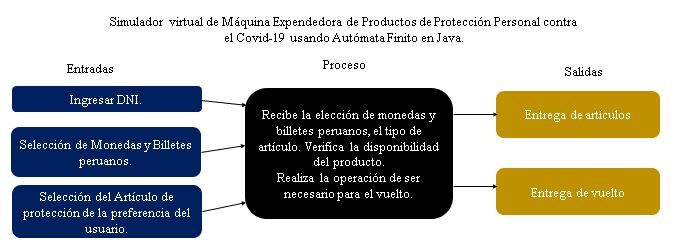
\includegraphics[width=9.5cm, height=3.5cm]{Diseño/Cajas Negras.JPG}
    \caption{Diagrama General de Cajas Negras.}
    \label{Caja1} 
    \vspace{1 mm}
    {\small Fuente: Elaboración propia.}
    \end{center}
    \end{figure}

\subsection{\underline{\textbf{Diseño detallado}}}

El simulador de Máquina Expendedora de Productos de Protección Personal contra el Covid-19 representada como modelo matemático, mediante un autómata finito no determinista, se muestra en la Figura ~\ref{Tec.5}, conformado por tres estados, el primero q0 como estado inicial, q1 como estado intermedio y q2 como estado final.

    \begin{figure}[H]
    \begin{center}
    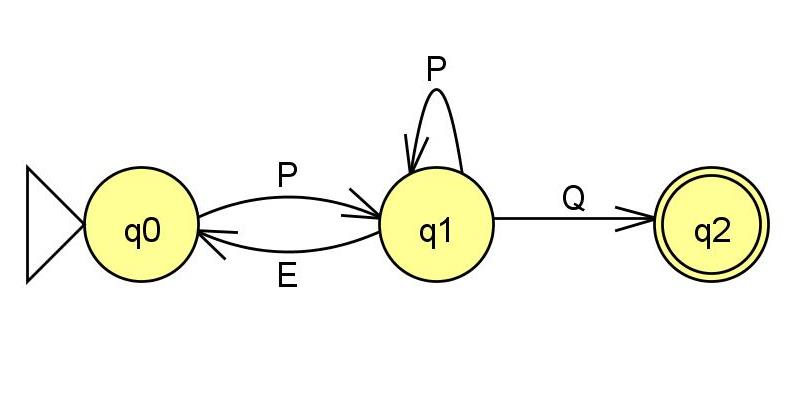
\includegraphics[width=7cm, height=3.3cm]{Diseño/PROCESO.jpg}
    \centering
    \caption{\small Autómata Finito No determinista empleado para el simulador virtual de Máquina Expendedora.}
    \label{Tec.5} 
    \end{center}
    \vspace{1 mm}
    {\small Fuente: Elaboración propia.}
    \end{figure}
    
Según la teoría de autómatas y lógica secuencial, la tabla de transición de estados correspondiente al autómata diseñado, se observa en la Tabla ~\ref{tab1}, que muestra en qué estado se moverá el autómata finito dado, basándose en el estado actual y las entradas.

%---------------------------------------------------------
\begin{table}[H]
\centering
\caption{Tabla de Transiciones de Estados para la Figura ~\ref{Tec.5}}
\label{tab1}
\begingroup
    \setlength{\tabcolsep}{10 pt} % Default value: 6pt
    \renewcommand{\arraystretch}{2} % Default value: 1
\begin{tabular}{|
>{\columncolor[HTML]{C0C0C0}}c |ccc|}
\hline
\cellcolor[HTML]{329A9D}{\color[HTML]{000000} } & \multicolumn{3}{c|}{\cellcolor[HTML]{329A9D}{\color[HTML]{000000} \textbf{\begin{tabular}[c]{@{}c@{}}Caracteres \\ de Entradas \end{tabular}}}} \\ \cline{2-4} 
\multirow{-2}{*}{\cellcolor[HTML]{329A9D}{\color[HTML]{000000} \textbf{Estados}}} & \multicolumn{1}{c|}{\cellcolor[HTML]{C0C0C0}{\color[HTML]{000000} \textbf{P}}} & \multicolumn{1}{c|}{\cellcolor[HTML]{C0C0C0}{\color[HTML]{000000} \textbf{Q}}} & \cellcolor[HTML]{C0C0C0}{\color[HTML]{000000} \textbf{E}} \\ \hline
{\color[HTML]{000000} \textbf{q0}} & \multicolumn{1}{c|}{{\color[HTML]{000000} q1}} & \multicolumn{1}{c|}{{\color[HTML]{000000} $\emptyset$}} & {\color[HTML]{000000} $\emptyset$} \\ \hline
{\color[HTML]{000000} \textbf{q1}} & \multicolumn{1}{c|}{{\color[HTML]{000000} q1}} & \multicolumn{1}{c|}{{\color[HTML]{000000} q2}} & {\color[HTML]{000000} q0} \\ \hline
{\color[HTML]{000000} \textbf{*qf}} & \multicolumn{1}{c|}{{\color[HTML]{000000} $\emptyset$}} & \multicolumn{1}{c|}{{\color[HTML]{000000} $\emptyset$}} & {\color[HTML]{000000} $\emptyset$} \\ \hline
\end{tabular}
\endgroup
\end{table}

\centering 
%\vspace{-3mm}
{Fuente: Elaboración propia.}
%---------------------------------------------------------
\justify 

\par 
Por lo tanto, según el diseño considerado en el proceso involucrado del Autómata Finito, su alfabeto se detalla en la Tabla ~\ref{tab3}, donde P, representa el dinero ingresado, por lo que se estableció que las monedas peruanas son: S/.1.00, Un Nuevo Sol; S/. 2.00, dos Nuevos Soles y S/. 5.00 Nuevos soles y billetes de S/.10.00 y S/.20.00 Nuevos soles y E representa el botón cancelar, que permitirá no efectuar la compra de algún articulo y así poder realizar otro proceso nuevamente o ya no realizar ninguno.

Además, Q, representa a los productos en el Autómata Finito, ver Tabla  ~\ref{tab2}, que cuenta dentro del simulador con características para ser identificados: ID, stock y precio de cada uno de las variables con las que cuenta el autómata.

\begin{table}[H]
\centering
\caption{Alfabeto}
\label{tab3}
\begingroup
    \setlength{\tabcolsep}{ 6pt} % Default value: 6pt
    \renewcommand{\arraystretch}{1.6} % Default value: 1
\begin{tabular}{|l|l|c|c|}
\hline
\multicolumn{1}{|c|}{\textbf{Entrada}} & \multicolumn{1}{c|}{\textbf{Descripción}} \\ \hline
\textbf{Q}                      & Productos del autómata (artículos de bioseguridad)                   \\ \hline
\textbf{P}                        &Inserción de dinero \\ \hline
\textbf{E}                        &Cancelación de la compra \\ \hline

\end{tabular}
\endgroup
\end{table}
\centering 
\vspace{-3mm}
{Fuente: Elaboración propia.}
\vspace{2mm}


\begin{table}[H]
\centering
\caption{Productos, Precios y Cantidad disponible}
\label{tab2}
\begingroup
    \setlength{\tabcolsep}{ 6pt} % Default value: 6pt
    \renewcommand{\arraystretch}{1.6} % Default value: 1
\begin{tabular}{|l|l|c|c|}
\hline
\multicolumn{1}{|c|}{\textbf{ID}} & \multicolumn{1}{c|}{\textbf{Producto}} & \textbf{Cantidad} & \textbf{Precio (Soles)} \\ \hline
\textbf{1}                        & Mascarilla quirúrgica                  & 10                & 0.50                    \\ \hline
\textbf{2}                        & Mascarilla KN95                        & 10                & 3.00                    \\ \hline
\textbf{3}                        & Alcohol en gel                         & 10                & 5.00                    \\ \hline
\textbf{4}                        & Alcohol 76°                            & 10                & 4.00                    \\ \hline
\textbf{5}                        & Protectores faciales                   & 10                & 8.00                    \\ \hline
\textbf{6}                        & Guantes                                & 10                & 1.00                    \\ \hline

\end{tabular}
\endgroup
\end{table}
\centering 
\vspace{-3mm}
{Fuente: Elaboración propia.}
\vspace{2mm}
\justify 

El simulador de Máquina Expendedora de Productos de Protección Personal contra el Covid-19 se da mediante una interfaz donde el usuario puede interactuar, la cual necesita la selección de monedas y billetes peruanos, entonces el proceso involucrado es:
\begin{enumerate}
    \item El usuario selecciona el dinero (monedas o billetes de denominación peruana (Nuevo Sol)), ver Figura ~\ref{sel_din} .
    
    \begin{figure}[H]
    \begin{center}
    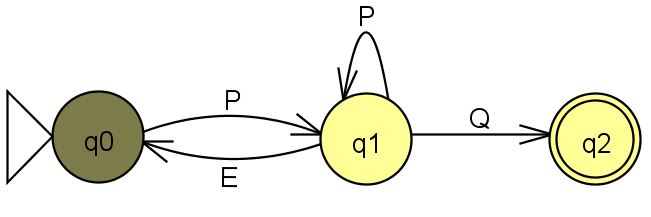
\includegraphics[width=8cm, height=2.5cm]{Diseño/Selec_dinero.JPG}
    \centering
    \caption{\small Autómata Finito No determinista en el estado donde se selecciona el dinero.}
    \label{sel_din} 
    \end{center}
    \vspace{1.5 mm}
    {\small Fuente: Elaboración propia.}
    \end{figure}

    \item El simulador verifica el dinero mediante el uso de estados.
    \item El usuario selecciona el Producto de Protección Personal contra el Covid-19 de su preferencia a comprar, ver Figura ~\ref{sel_prod}.
    
    \begin{figure}[H]
    \begin{center}
    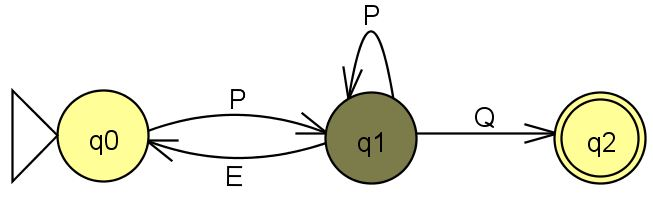
\includegraphics[width=8cm, height=2.5cm]{Diseño/Selec_produ.JPG}
    \centering
    \caption{Autómata Finito No determinista en el estado donde se selecciona el producto.}
    \label{sel_prod} 
    \end{center}
    \vspace{1.5 mm}
    {\small Fuente: Elaboración propia.}
    \end{figure}

    \item El simulador verifica si hay disponibilidad dentro del stock del producto seleccionado.
    \item El usuario selecciona el botón 'Comprar', ver Figura ~\ref{comrpa}.
    
    \begin{figure}[H]
    \begin{center}
    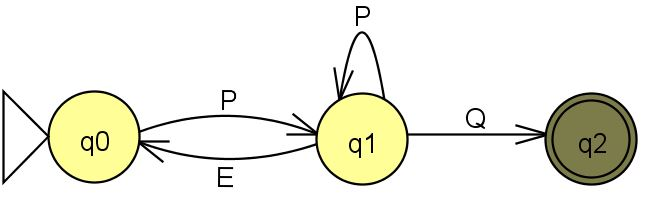
\includegraphics[width=8cm, height=2.5cm]{Diseño/Compra.JPG}
    \centering
    \caption{Autómata Finito No determinista en el estado donde se selecciona el botón comprar.}
    \label{comrpa} 
    \end{center}
    \vspace{1.5 mm}
    {\small Fuente: Elaboración propia.}
    \end{figure}
    
    \item Si el vuelto existe, ir a paso 7.
    \item Se imprimirá el mensaje "Vuelto entregado".
    \item El producto se compra y aparece el mensaje impreso: " Gracias por la compra", y finaliza el proceso.
    \item El producto y la cantidad de dinero seleccionado puede cancelarse y evitar finalizar la adquisición de la compra, mediante el botón Cancelar".
\end{enumerate}


\section{\textbf{Análisis de resultados}}

\subsection{\underline{\textbf{Resultados obtenidos}}}
Para la implementación realizada en el lenguaje de programación Java, hemos considerado una base de datos de clientes frecuentes, donde se almacena, sus nombres y apellidos, DNI y cantidad de compras realizadas, a continuación las principales interfaces de cada etapa del proceso y el funcionamiento del simulador de la Máquina Expendedora de Productos de Protección Personal contra el Covid-19.

\begin{figure}[H]
    \begin{center}
    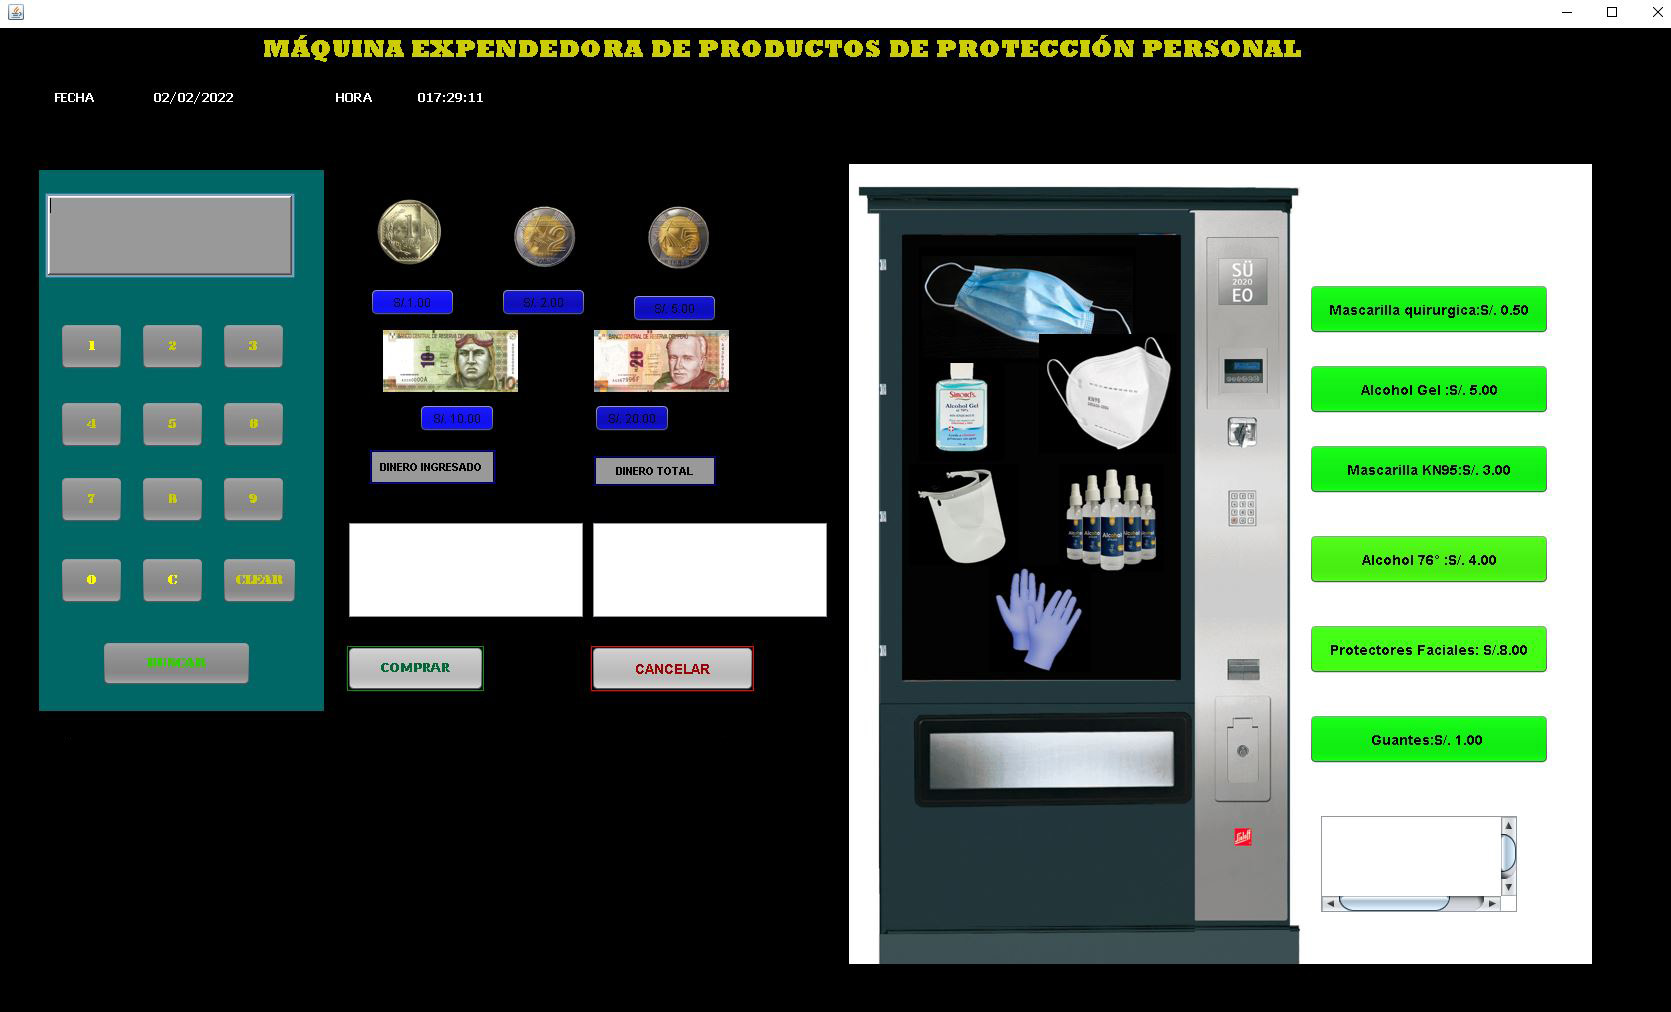
\includegraphics[width=8cm, height=5cm]{Resultados/1-Interfaz.JPG}
    \centering
    \caption{Interfaz Principal, al abrir el simulador.}
    \label{1-Interfaz} 
    \vspace{1.5 mm}
    {\small Fuente: Elaboración propia, extraída del entorno NetBeans para lenguaje de programación Java.}
    \end{center}
\end{figure}

Obsérvese en la Figura ~\ref{1-Interfaz}, la cual muestra una pantalla gris a lado izquierdo, donde mostrará el DNI del usuario y un teclado virtual en el que se ingresará este, además en la parte central se observa las monedas y billetes a usar, también los botones comprar y cancelar y dos espacios en blanco en los cuales se mostrará la cantidad de dinero ingresado y el total. Por otro lado tenemos la visualización de los productos y los nombres y precios de los productos.

\begin{figure}[H]
    \begin{center}
    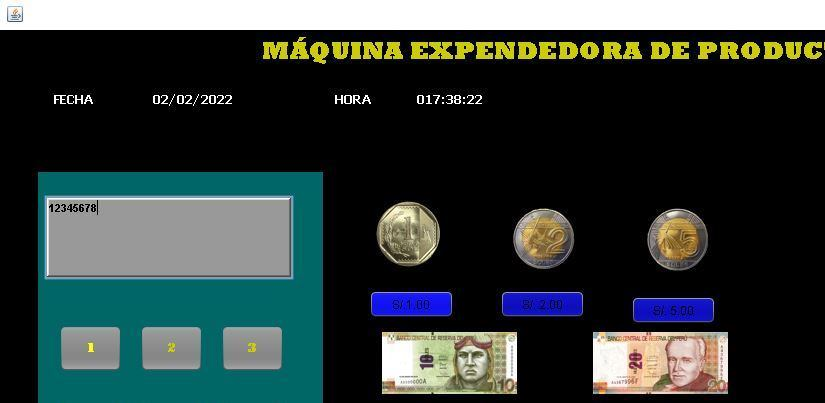
\includegraphics[width=8cm, height=3.5cm]{Resultados/2-Interfaz.JPG}
    \centering
    \caption{Interfaz Principal, digitando DNI.}
    \label{2-Interfaz} 
    \vspace{1.5 mm}
    {\small Fuente: Elaboración propia, extraída del entorno NetBeans para lenguaje de programación Java.}
    \end{center}
\end{figure}

Obsérvese de la Figura ~\ref{2-Interfaz} en la pantalla gris izquierda el DNI ingresado, en este caso '12345678', como ejemplo para la explicación.

\begin{figure}[H]
    \begin{center}
    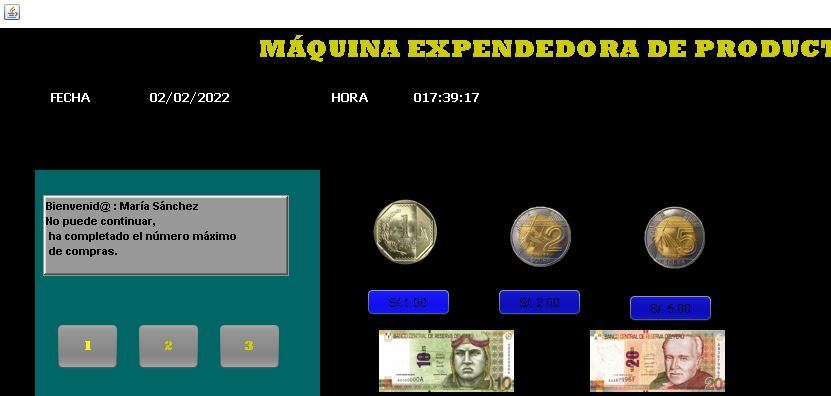
\includegraphics[width=8cm, height=3.5cm]{Resultados/3-Interfaz.JPG}
    \centering
    \caption{Interfaz Principal, bienvenida al usuario y restricción por máximo de compras.}
    \label{3-Interfaz} 
    \vspace{1.5 mm}
    {\small Fuente: Elaboración propia, extraída del entorno NetBeans para lenguaje de programación Java.}
    \end{center}
\end{figure}

Obsérvese en la Figura ~\ref{3-Interfaz} que luego de haber ingresado el DNI y darle clic al botón 'BUSCAR', se mostrará en dicha pantalla el nombre: 'María Sánchez' y que el usuario ha completado el máximo de compras, la cual es mayor a 5 compras, por lo que el simulador no le permitirá realizar ninguna compra. Por lo tanto, los botones de comprar y cancelar, a su vez de seleccionar monedas, billetes y productos estarán inhabilitados.

\begin{figure}[H]
    \begin{center}
    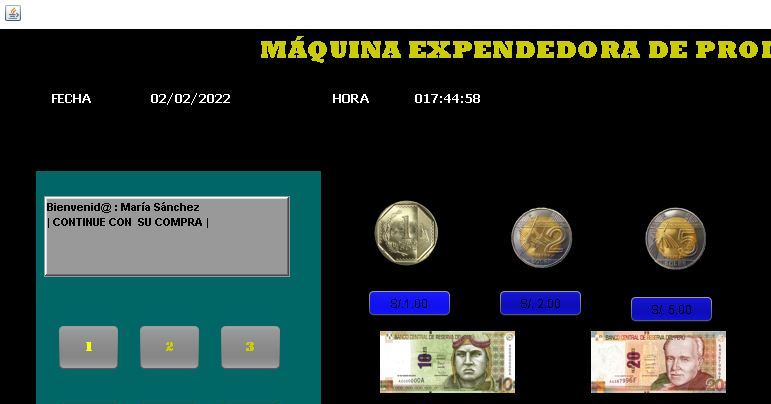
\includegraphics[width=8cm, height=3.5cm]{Resultados/4-Interfaz.JPG}
    \centering
    \caption{Interfaz Principal, bienvenida al usuario e indicación que puede continuar su compra.}
    \label{4-Interfaz} 
    \vspace{1.5 mm}
    {\small Fuente: Elaboración propia, extraída del entorno NetBeans para lenguaje de programación Java.}
    \end{center}
\end{figure}

Obsérvese en la Figura ~\ref{4-Interfaz} que, luego de haber ingresado su DNI y el simulador al reconocer que el usuario no ha completado su número máximo de compras puede continuar con la adquisición de cualquier producto, para la explicación se continuará con el nombre de 'María Sánchez'.

\begin{figure}[H]
    \begin{center}
    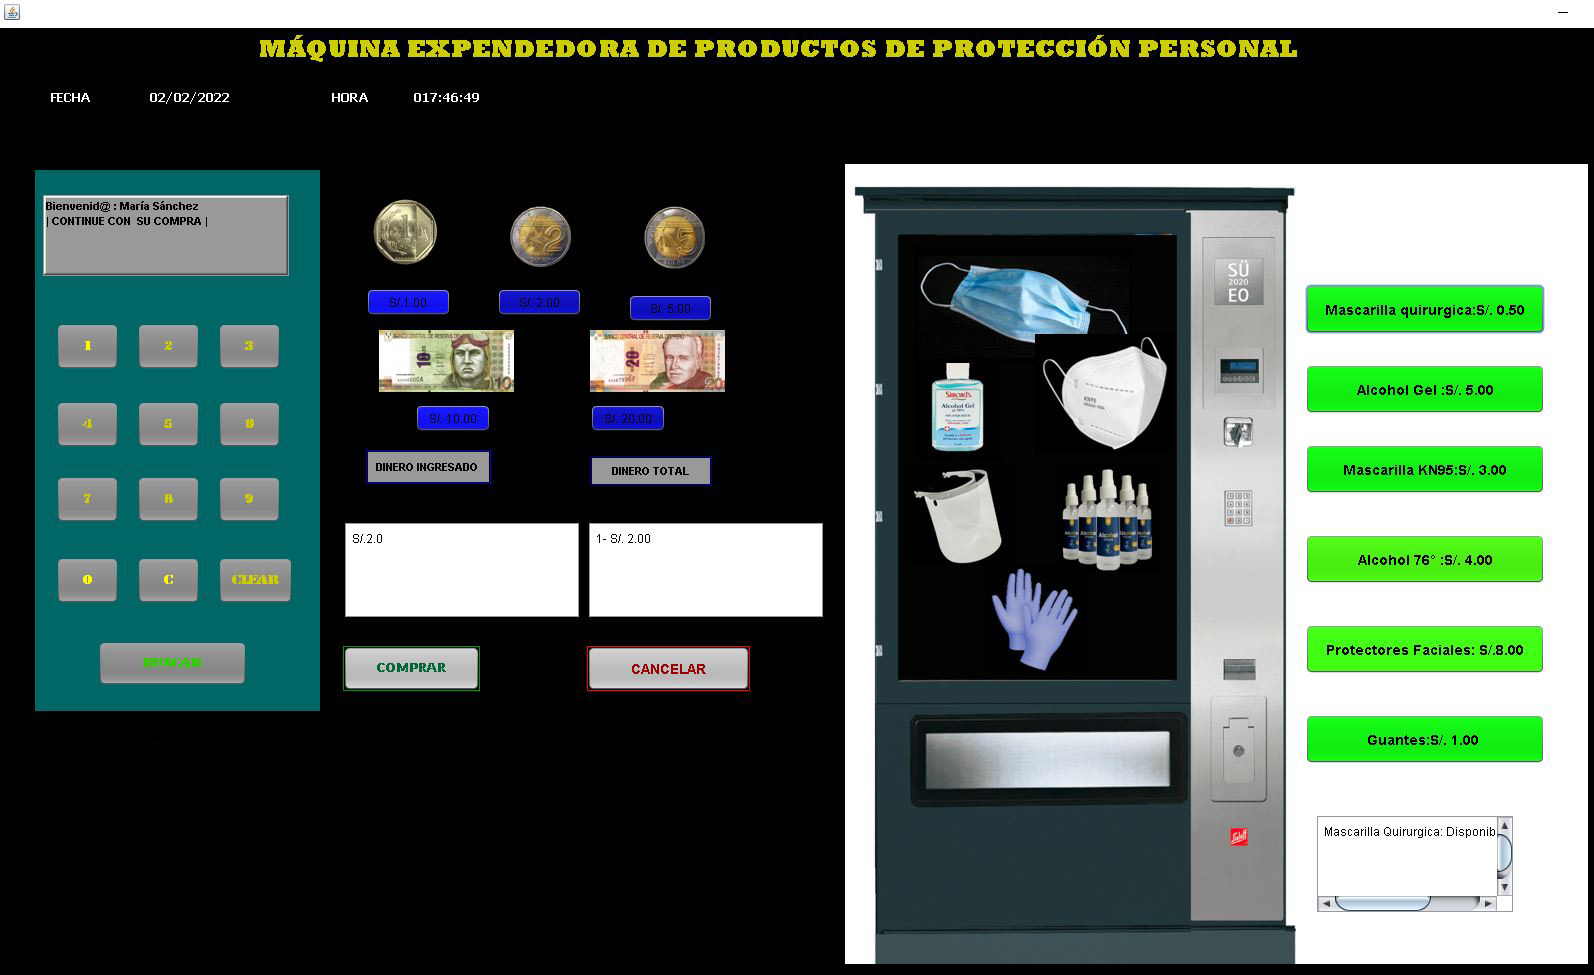
\includegraphics[width=8cm, height=5cm]{Resultados/5-Interfaz.JPG}
    \centering
    \caption{Interfaz Principal, selección de monedas/billetes y producto, estando en q1.}
    \label{5-Interfaz} 
    \vspace{1.5 mm}
    {\small Fuente: Elaboración propia, extraída del entorno NetBeans para lenguaje de programación Java.}
    \end{center}
\end{figure}
\begin{figure}[H]
    \begin{center}
    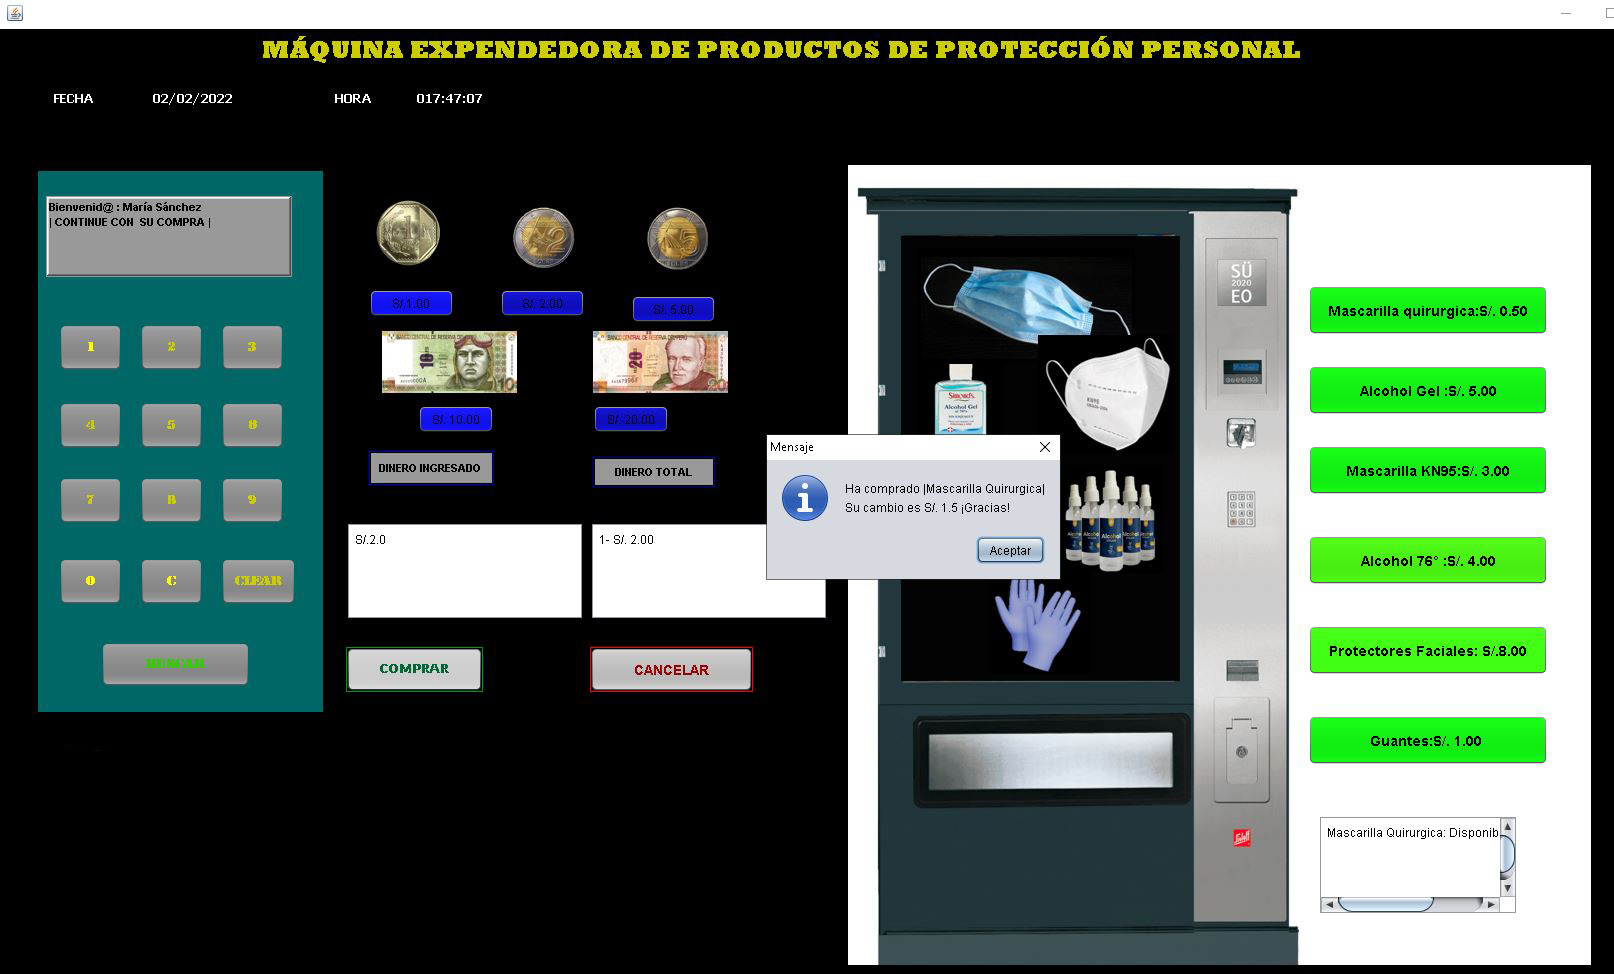
\includegraphics[width=8cm, height=5cm]{Resultados/6-Interfaz.JPG}
    \centering
    \caption{Interfaz Principal, realización de la compra, estando en q2(estado final).}
    \label{6-Interfaz} 
    \vspace{1.5 mm}
    {\small Fuente: Elaboración propia, extraída del entorno NetBeans para lenguaje de programación Java.}
    \end{center}
\end{figure}

Obsérvese en la Figura ~\ref{5-Interfaz} que, el usuario selecciona, en este caso una moneda de S/.2.00 soles, y a su vez el producto de Mascarilla Quirúrgica que tiene por precio S/.0.50 céntimos, por lo que el estado en el Autómata Finito cambia a q1; y en la Figura ~\ref{6-Interfaz} se observa que luego de dar clic al botón 'COMPRAR', aparece una subventana donde se muestra el cambio si es fuese el caso o que la compra está realizada y el estado en el Autómata Finito cambia a q2 (estado final).

\subsection{\underline{\textbf{Discusión}}}

El simulador de Máquina Expendedora de Productos de Protección Personal contra el Covid-19 implementado genera interacción con el usuario, evidenciando el proceso que realiza el autómata finito no determinista, con la finalidad de evitar aglomeraciones y contagios entre los ciudadanos, el cuál a través de la selección de monedas y billetes se realiza la compra y venta de artículos de protección y calcula el vuelto a ser entregado. 

De forma similar, \citeA{indo}, en su Aplicación del concepto de autómatas de estado finito en aplicaciones de simulación de máquinas expendedoras de arroz, en medio de la actual pandemia de coronavirus (COVID-19) debido a que la gente tiene miedo de ir al mercado porque el mercado es uno de los grupos más grandes de Covid-19 y se espera que sea una de las soluciones para detener la propagación y transmisión de COVID-19, diseñó y estableció una simulación de máquina virtual de arroz que puede vender automáticamente arroz ingresando en forma de papel moneda o con dinero electrónico y la salida en forma de recibo de compra de arroz con 5 tipos de arroz. 

Igualmente que el presente artículo, el método utilizado es Autómata de Estado Finito (FSA) tipo Autómata de Estado Finito No Determinista (NFA) el cual se define por cinco tuplas, con la fórmula: $M = (Q, \Sigma, \delta, S, F)$, se eligió NFA porque puede explicar el concepto de trabajo en detalle para que sea fácil de entender y los resultados de la FSA se puedan convertir en conceptos lógicos simples para la implementación.

\section{\textbf{Conclusiones}}
Se desarrolló un prototipo de simulador virtual de una Máquina Expendedora de Productos de Protección Personal contra el Covid-19 utilizando un Autómata Finito No determinista, usando el lenguaje de programación Java con el IDE Netbeans 8.2, que está conformado por tres estados, tres elementos de su alfabeto, para la adquisición de artículos de bioseguridad manteniendo el cuidado personal de los habitantes y evitar la propagación de este virus y la usura en los precios de estos ante la actual crisis sanitaria en Perú causada por el Covid-19.
\\
Se ha evidenciado y probado la importancia de la Teoría de Autómatas y Lenguajes Formales para el desarrollo de ideas para el contexto de pandemia.
\\
Se ha tomado en cuenta la eficacia de autómatas para el proceso que asume y la creación de una máquina expendedora.
\\
Se ha recreado esta idea de simulación para la ayuda de prevención contra la pandemia de Covid - 19 evitando el contacto físico con otras personas.

%--------------------------------------------------------------------
\bibliographystyle{apacite}
\bibliography{Referencias}

\end{document}